\newpage
\section{Task 3: Entity-Relationship modelling}

You have been hired to design a database system for a pizza store. The database must encompass the customers, staff, pizza details and the pizza orders made by customers.

\subsection{Assumptions}

\begin{itemize}
\item A customer must order at least one pizza to exist on database
\item Some staff may not take any CustomerOrders
\item A CustomerOrder must contain at least one PizzaOrder
\item A PizzaOrder must include one PizzaType selection
	\begin{itemize}
	\item It is possible that a PizzaType may never be selected for a PizzaOrder
	\end{itemize}
\item A PizzaOrder must include one PizzaCrust selection
	\begin{itemize}
	\item It is possible that a PizzaCrust may never be selected for a PizzaOrder
	\end{itemize}
\item A PizzaOrder must include one PizzaSauce selection
	\begin{itemize}
	\item It is possible that a PizzaSauce may never be selected for a PizzaOrder
	\end{itemize}
\end{itemize}

\subsection{Logical E-R diagram}

\begin{figure}[H]
\centering
\caption{Pizza Store Logical E-R Diagram}
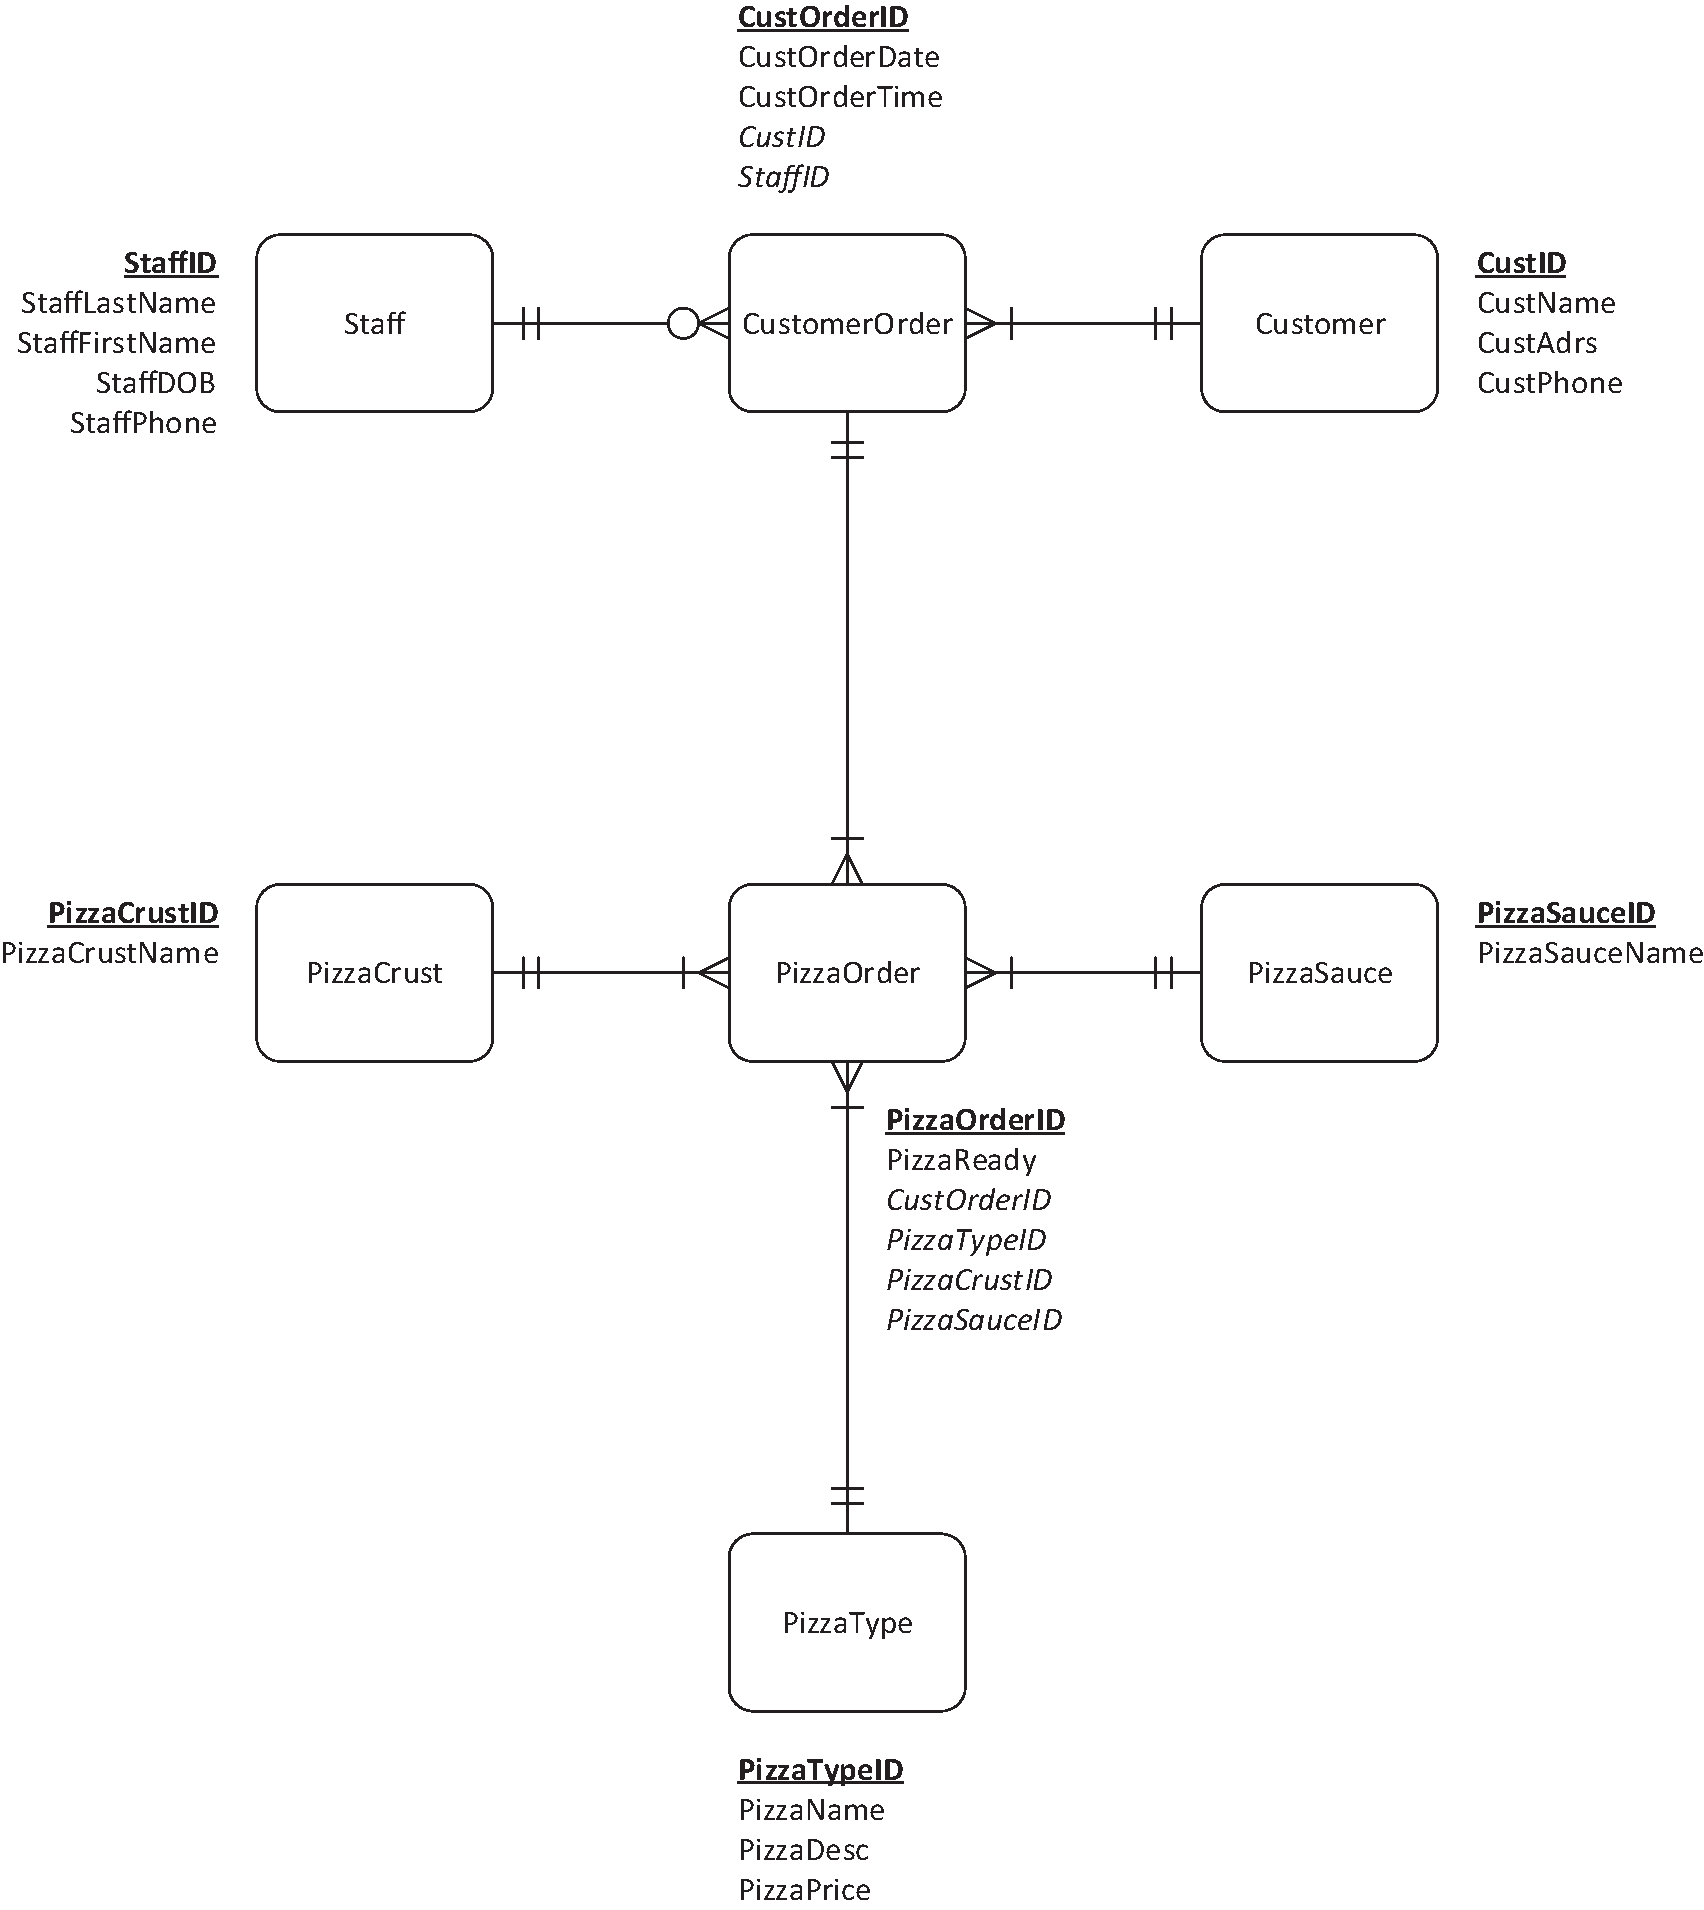
\includegraphics[scale=0.5]{./img/CSG1207_A1_PONCE_TASK_3_LER_PIZZA.pdf}
\end{figure}

\subsection{Physical E-R diagram}

\begin{figure}[H]
\centering
\caption{Pizza Store Physical E-R Diagram}
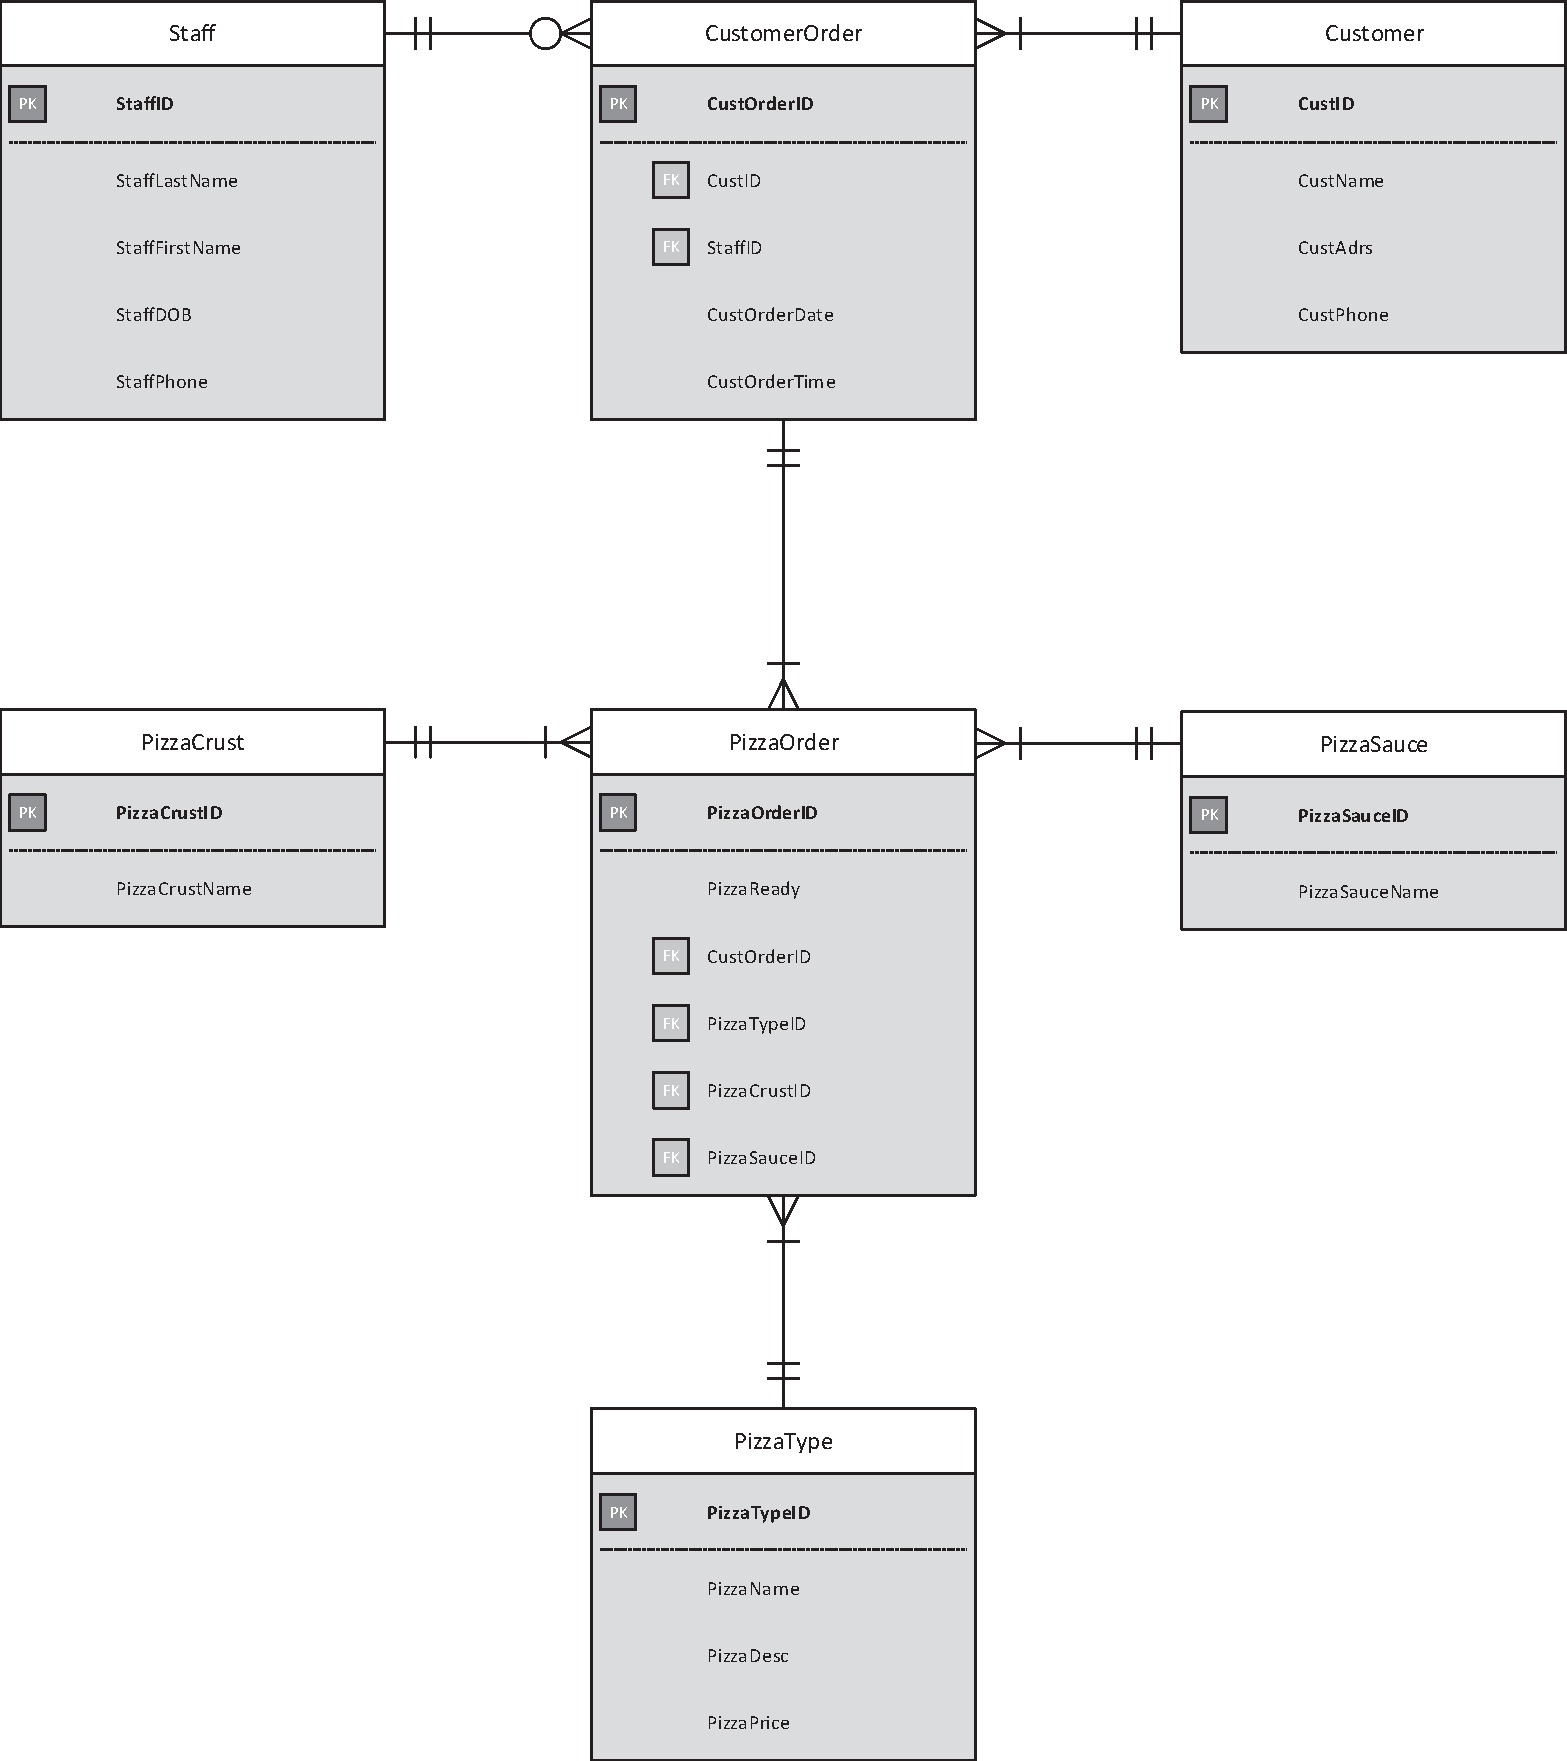
\includegraphics[scale=0.5]{./img/CSG1207_A1_PONCE_TASK_3_PER_PIZZA.pdf}
\end{figure}